\chapter{Inference through forward linear regression}
Let us suppose that the observed data are produced by an autonomous system of equations of the form, with a multiplicative stochastic noisec term:
\begin{equation*}
    \dot{x}_i = F(x) + x_i\cdot \sigma \cdot \eta_i
\end{equation*}
where the model $f(x)$ is unknown and $\eta_i$ is a normally distributed random variable with zero mean and unit variance. Let us also make the (strong) assumption that the observed data evolves closely to a steady state $x^{*}, f(x^{*}) = 0$. Under the latter assumption, we can linearize the system around the equilibrium:

\begin{equation*}
    \dot{x}_i(t) = J_{F}(x^{*})\cdot (x-x^*) + o(||x- x^*||) + + x_i^*\cdot \sigma \cdot \eta_i
\end{equation*}
the jacobian $J_{F}(x^{*})$ is the so-called community matrix at the equilibrium $x^*$.


This method essentially consists in inferring the $i- th$ row of the community matrix through a least squares regression of the derivative $\dot{x_i}$ (covariate variable) versus the abundances $\{(x_j - x_j^{*})\}_{j=1}^{N}$.
The compositional constraint on the abundances $(\sum_i\, x_i(t) \equiv 1 \,\quad \forall \,t)$, poses a technical difficulty, as the design matrix is singular and hence, the usual least squares regression has no unique solution. To bypass this problem, a forward step regression can be performed instead, which also has the benefit of promoting sparsity. Forward stepwise regression consists in adding one regressor at each step, up to a maximum of $(N-1)$ regressors. By doing this, the columns of the design matrix are always linearly independent. The dataset is first divided into two disjoint subsets: a training dataset and a test dataset. Then, one step of the algorithm works like this:
\begin{enumerate}
    \item For each possible new regressor, the least squares fit is performed on the training dataset
    \item the performance (MSE) of the fits are evaluated on the test dataset
    \item  The new regressor is chosen as the one for which the fit gives the best performance on the test dataset
\end{enumerate}
This basic step is repeated until either the fit improvement falls below a pre-specified threshold, or the maximum number of regressors is reached.

Computational cost can be a concern for this method: in the worst case scenario, the inference of the $i-th$ row requires repeating the least suqares regression $(N-1)$ times. So the overall cost scales as $\sim N^2 \cdot$ cost of one single least squares.

Also, one should account for the error-in-variables problem and the collinearity of the covariate and the regressors.
The covariates $\dot{x_i(t)}$ can be estimated through finite differences:
\begin{equation*}
    \dot{x}_i = \frac{x_i(t+\Delta\,t) - x_i(t)}{\Delta t}
\end{equation*}
or 
\begin{equation*}
    \dot{x}_i = \frac{x_i(t+\Delta\,t) - x_i(t-\Delta t)}{2\,\Delta t} 
\end{equation*}
or higher order formulas.
Clearly, for these numerical estimations to be precise, the time interval $\Delta t$ between consecutive measures needs to be sufficiently small. Otherwise, the data should be interpolated, but this introduces a bias. 


\section{Results with simulated data}

The data 

Una prova su dati simulati che effettivamente evolvono attorno all'equilibri, quindi soltanto per controllare se l'algoritmo funziona come deve. 
La regressione con le derivate inferisce la matrice jacobiana all'equilibrio (community matrix), che per il LV è $J_{i,\,j} = a_{i,j}\cdot \overline{x}_i$, metren la regressione con il modello proposto da fisher inferisce direttamente la matrice delle interazioni, moltiplicata per l'intervallo tra due misure consecutive: $a_{i,j}\cdot \Delta_t$. 
\begin{figure}[H]
    \centering
    \subfigure[]{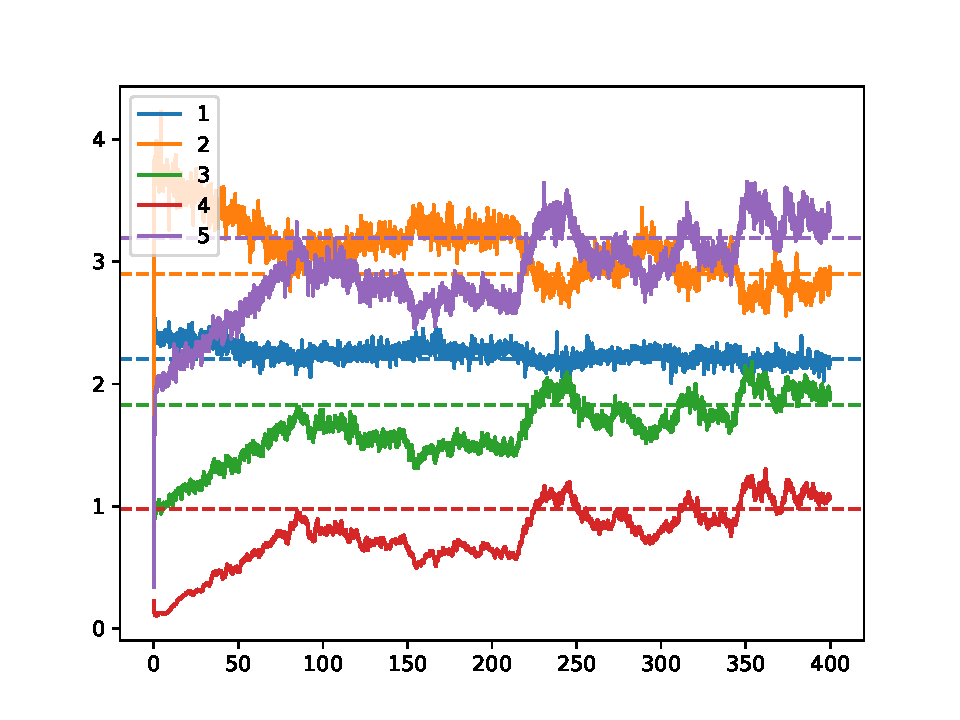
\includegraphics[width=0.7\linewidth]{figures/chapter_3/regression/timeseries_2024-08-24_17-29-06.pdf}}
    \subfigure[]{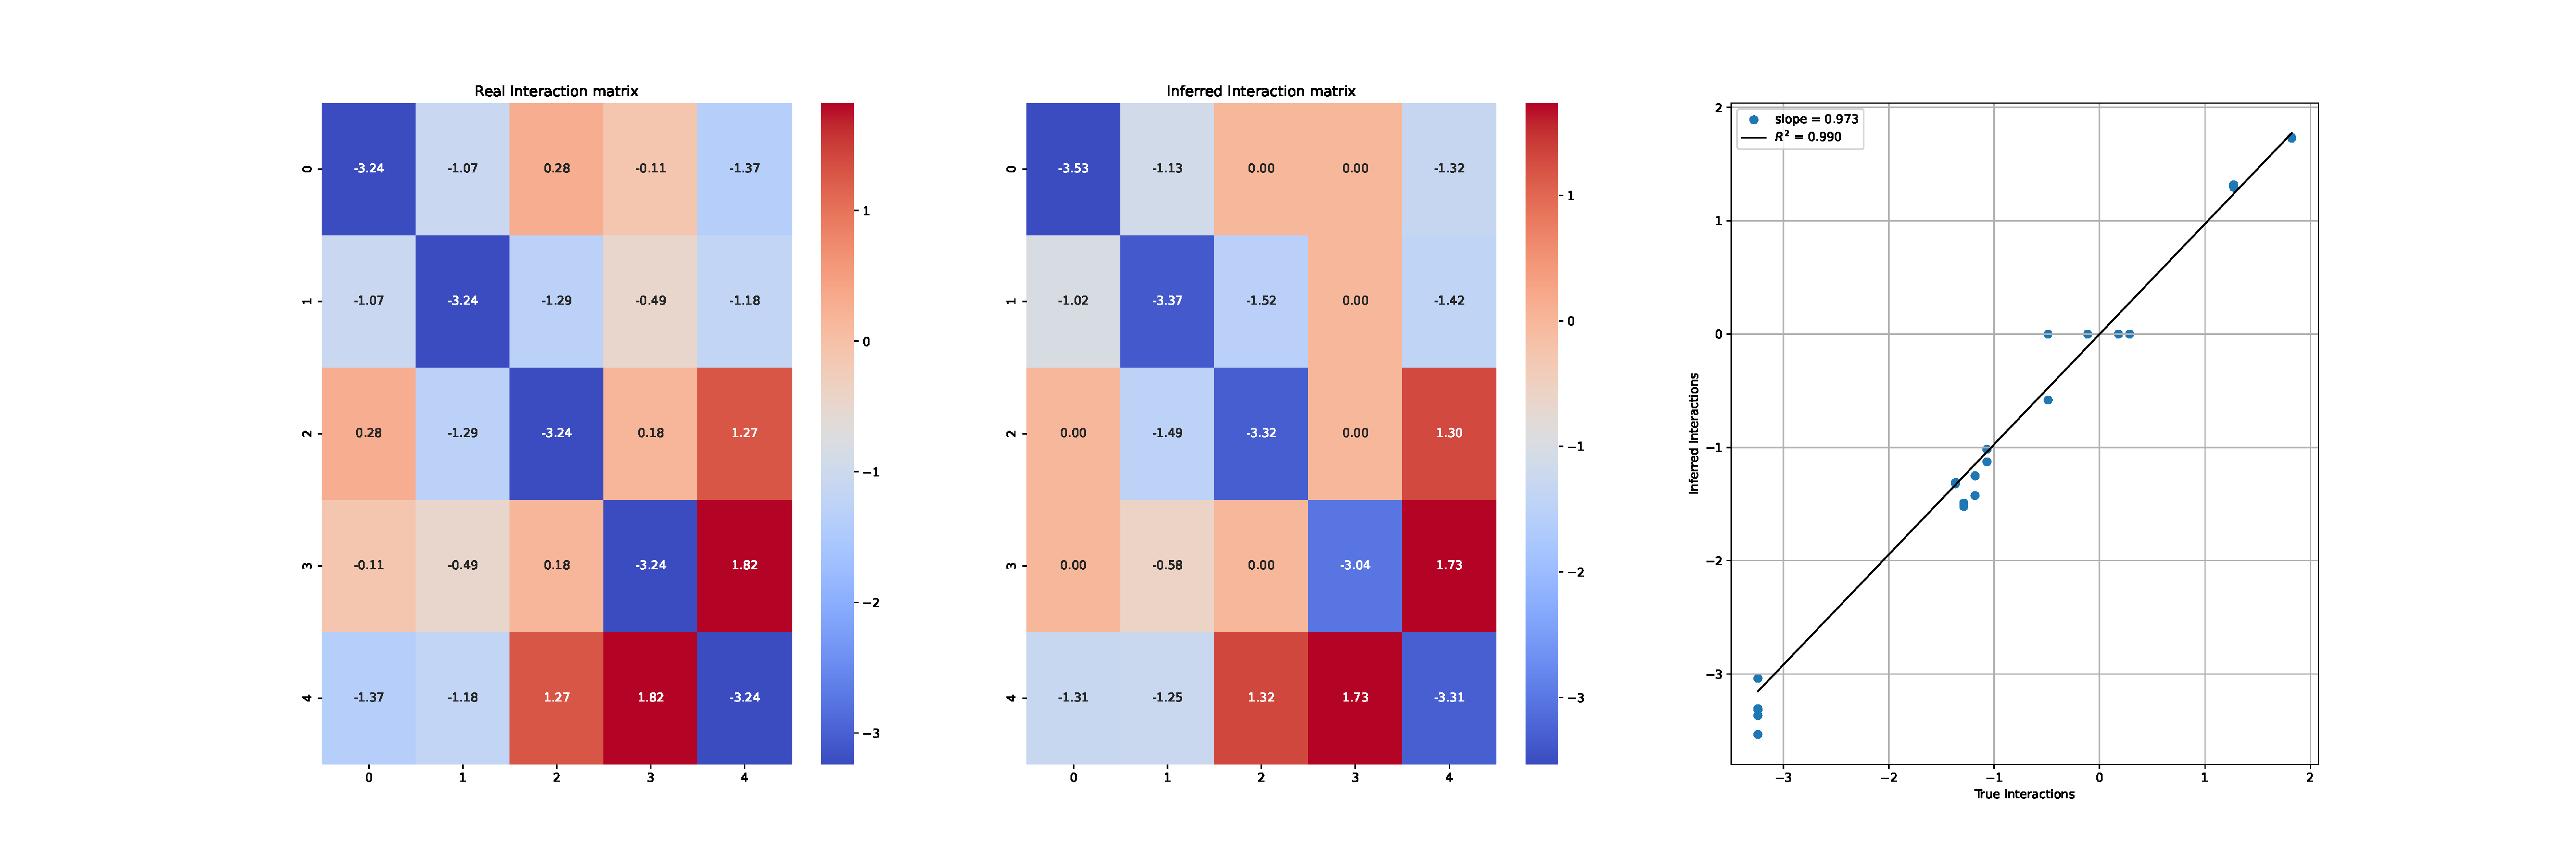
\includegraphics[width=\linewidth]{figures/chapter_3/regression/matrix_comparison_2024-08-24_17-31-23.pdf}}
    \subfigure[]{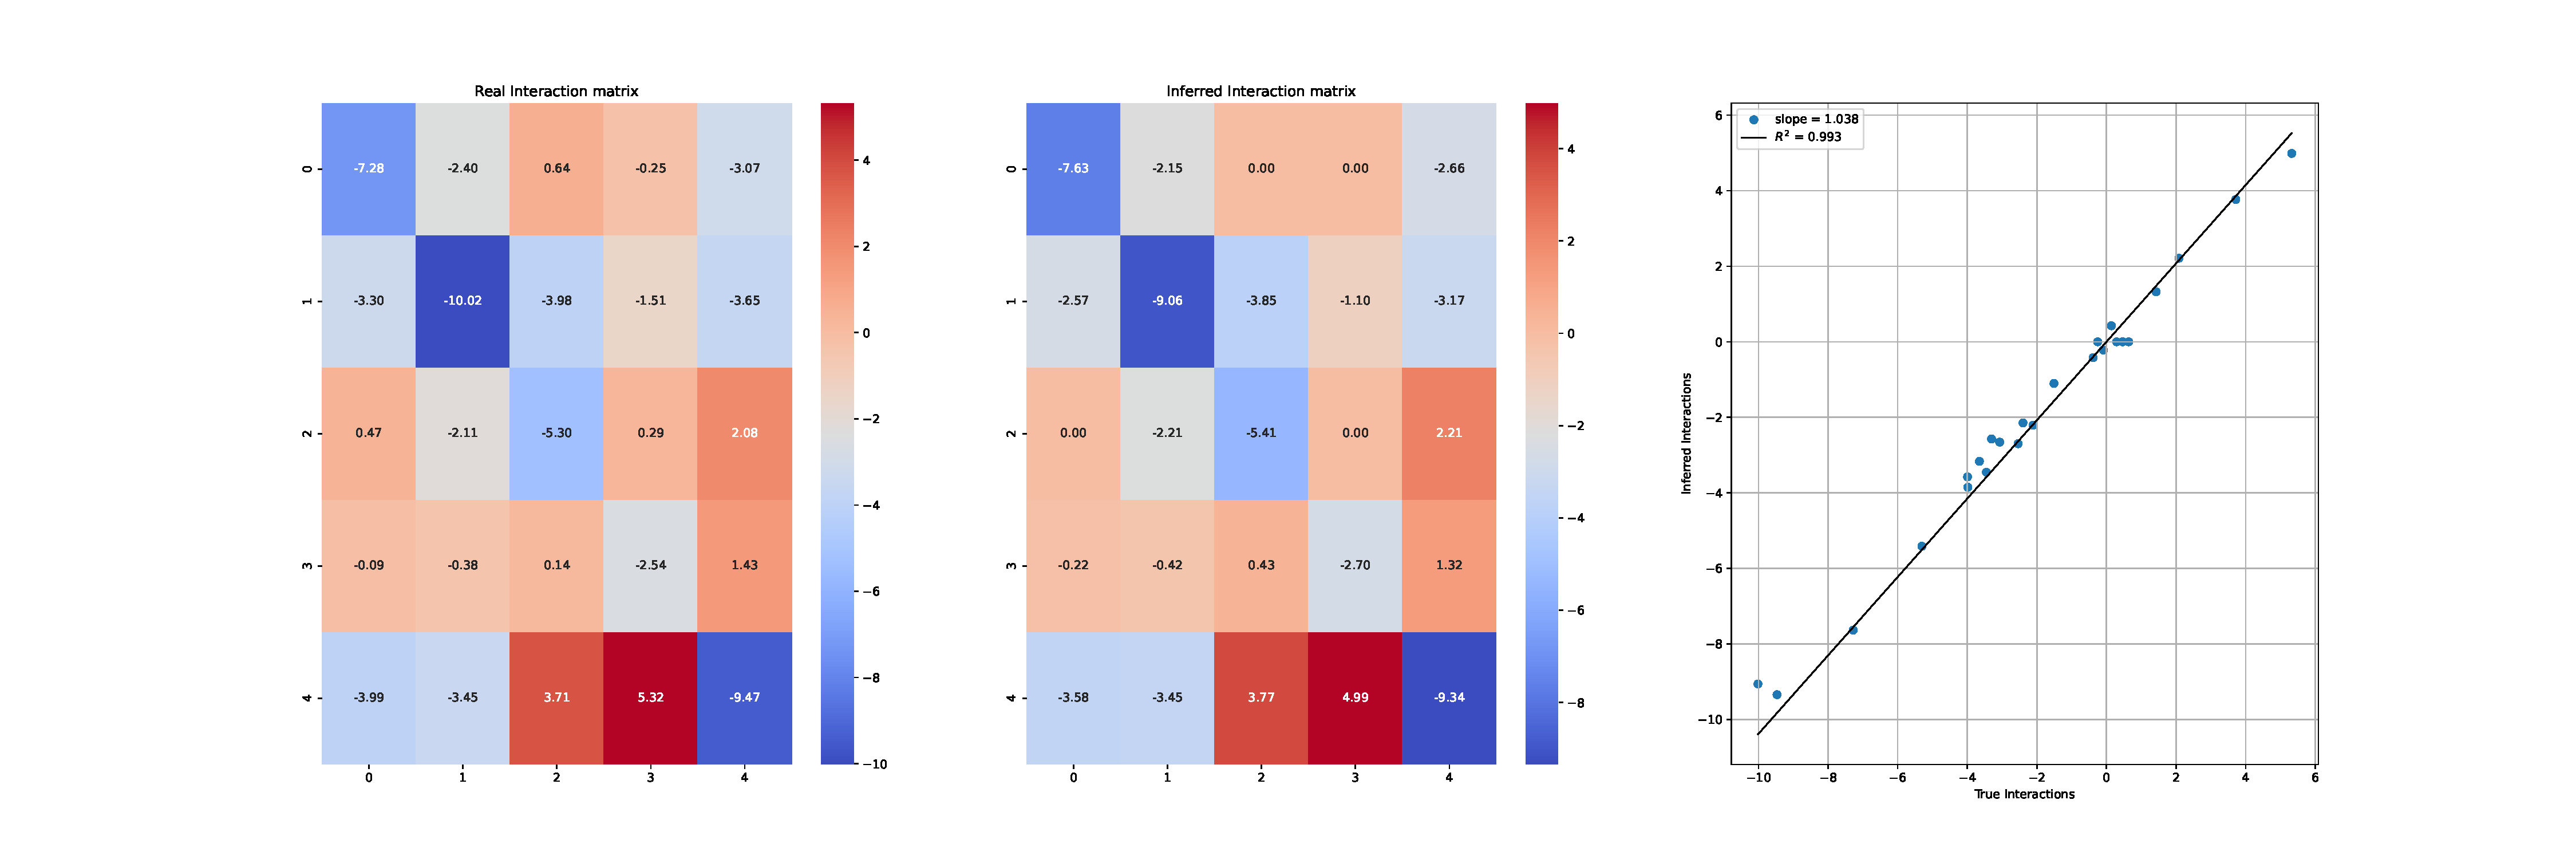
\includegraphics[width=\linewidth]{figures/chapter_3/regression/matrix_comparison_2024-08-24_17-31-24.pdf}}
    \caption{Fig (a): Qui ci sono $5$ specie, giorni $400$, sampling rate $100$ misure al giorno, $sigma=5$. Soglia impostata a $0.1\%$ e numbero di bagging $100$. (Fig. b) metodo di fisher, matrice delle interazioni $a_{i,j}$ reale (sx) e inferita (dx), (Fig. c) classica regressione sulle derivate, matrice di comunità $(J_{i,\,j} = a_{i,\,j}\cdot \overline{x}_i)$ reale e inferita. Performance buone e grossomodo paragonabili. Ci mancherebbe! Se non funzionasse nemmeno su questi dati sarebbe completamente inutile.}
    \label{fig:enter-label}
\end{figure}

\section{Results on mice data}

The method proposed in \parencite{fisher} assumes that:
\begin{enumerate}
\item the observed data is well described by a generalized Lokta-Volterra model, with discrete timesteps and a stochastic noise term,
\item in particular, the observed data is a trajectory in the neighbourhood of a \textbf{stable} (locally? globally? not clear from the paper, but not crucial) and \textbf{feasible} equilibrium $\overline{x}$ The equilibrium values $\overline{x_i}$ can be directly inferred from the data by taking the median (\textcolor{orange}{or mean}) of the abundaces.
\end{enumerate}

The discrete stochastic Lokta Volterra equation is the following:

\begin{equation}
\label{eq:Fisher}
x_i(t + \Delta t^{\small update}) = \eta_i(t) \cdot x_i(t) \cdot \exp \left[ \Delta t^{\small update} \sum_{j=1}^{N} C_{ij} \left[ x_j(t) - \bar{x}_j \right] \right]
\end{equation}

$\eta_i(t)$ is a lognormally distributed variable, representing a stochastic noise. The reason why it is assumed lognormal is that when taking the logaritm we get a normally distributed noise $\eta_i(t) \sim \mathcal{N}(0, \sigma).$ \\
\newline
\begin{equation}
\ln\left[x_i(t + \Delta t^{\small update})\right] - \ln\left[x_i(t)\right] = \zeta_i(t) + \Delta t^{\small update} \sum_{j=1}^{N} C_{ij} \left[ x_j(t) - \bar{x}_j \right]
\end{equation}
Equations \ref{eq:Fisher} simplify to:
\begin{equation*}
    \centering
     \dot{x}_i(t) = x_i(t)\cdot \left[\sum_j\, c_{i,\,j}\, \left(x_j- \overline{x}_j\right)\right]
\end{equation*}
in the limit case $\Delta\, t^{(sampling)}\rightarrow 0$ and $\eta_i(t) \equiv 0$. One can recast these equations into the usual Lokta Volterra equations $ \dot{x}_i(t) = x_i(t)\cdot \left[ r_i\, + \sum_j\, a_{i,\,j}\, x_j \right]$, by identifying
\begin{equation*}
     a_{i,\,j} \equiv c_{i,\,j} \quad \text{and} \quad r_i \equiv - \sum_j\, c_{i,\,j}\,\overline{x}_j
\end{equation*}
$[Ax + r]\overline{x} = 0$ is indeed a necessary condition that must be satisfied by  a feasible equilibrium.





\section{Performance evaluation with simulated data}
Parameters of the simulation are: sampling matrix $C$, sampling rate $m$, noise $\sigma$.
In the code, the entries of the interaction matrix are normalized to unity. In all the following simulations, the entries of the interaction matrix, $c_{i,j}$ are normalized to unity. Re-scaling the interactions is perfectly equivalent to rescaling the update interval, keeping the other parameters fixed.
A possibility must be considered that the update time scale of the evolution process is different from the time scale of the sampling, most likely smaller. In fact, the experimental measures might be taken at consecutive steps $\Delta\,t^{\small (sampling)} = m\cdot \Delta\, t^{\small update}$, where $m > 0$ is an integer multiplying $\Delta t$. For example, it might that the data is well described by a gdLV assuming a timescale is in the order of magnitude of hours, while the measurements are only made each few days. In this case, the accuracy of the fit might well be low. A partial solution, in order to still apply the method when $\Delta t^{(\small sampling)} > \Delta t^{(\small update)}$ is to interpolate the missing experimental values in order to obtain a timeseries where $m = 1$. Of course, the more the two timescales differ, the least this approximation will work. Since we do not know the process timescale in advance when approaching data, we shall try by guess and then compare the results. \textcolor{red}{Question for professors:} what is the expected time scale of bacteria reproduction?
\\

One issue arising with relative abundances data is that a value of zero counts is ambiguous: one cannot known if the species is truly absent, or just so low in abundance that it does not apppear in the sample. 

The fact that the covariate in the regression is a logarithm $y_i = log(x_i t +1) - log(x_i t)$ induces the need to discard all the timepoints where there are zero counts. This makes the inference of interactions impractical for species like those plotted in \ref{fig:rare_species}. For this method is hence reasonable to select the most abundant species with respect to the median counts instead of the mean counts.

Thing to check in simulations are:

\begin{enumerate}
    \item performance at variying threshold on fit improvement,
    \item performance at varying species number $N$,
    \item performance at varying stochasticity level $\sigma$
\end{enumerate}



\begin{figure}[H]
\centering
\subfigure[]{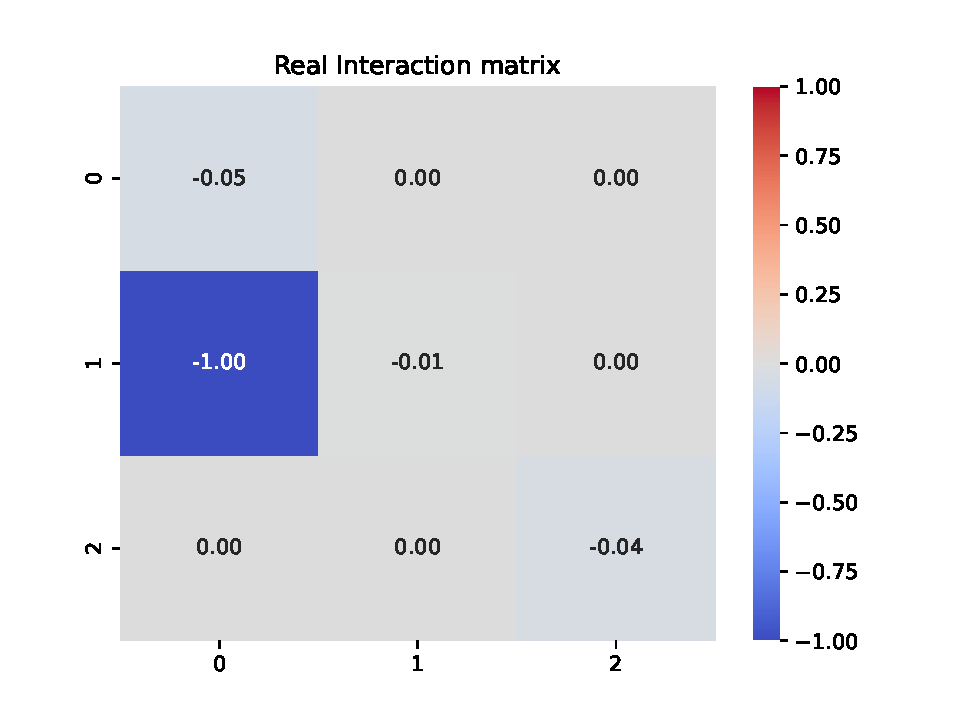
\includegraphics[width = 0.25\linewidth]{figures/chapter_3/matrix_3.pdf}}
\hfill
\subfigure[]{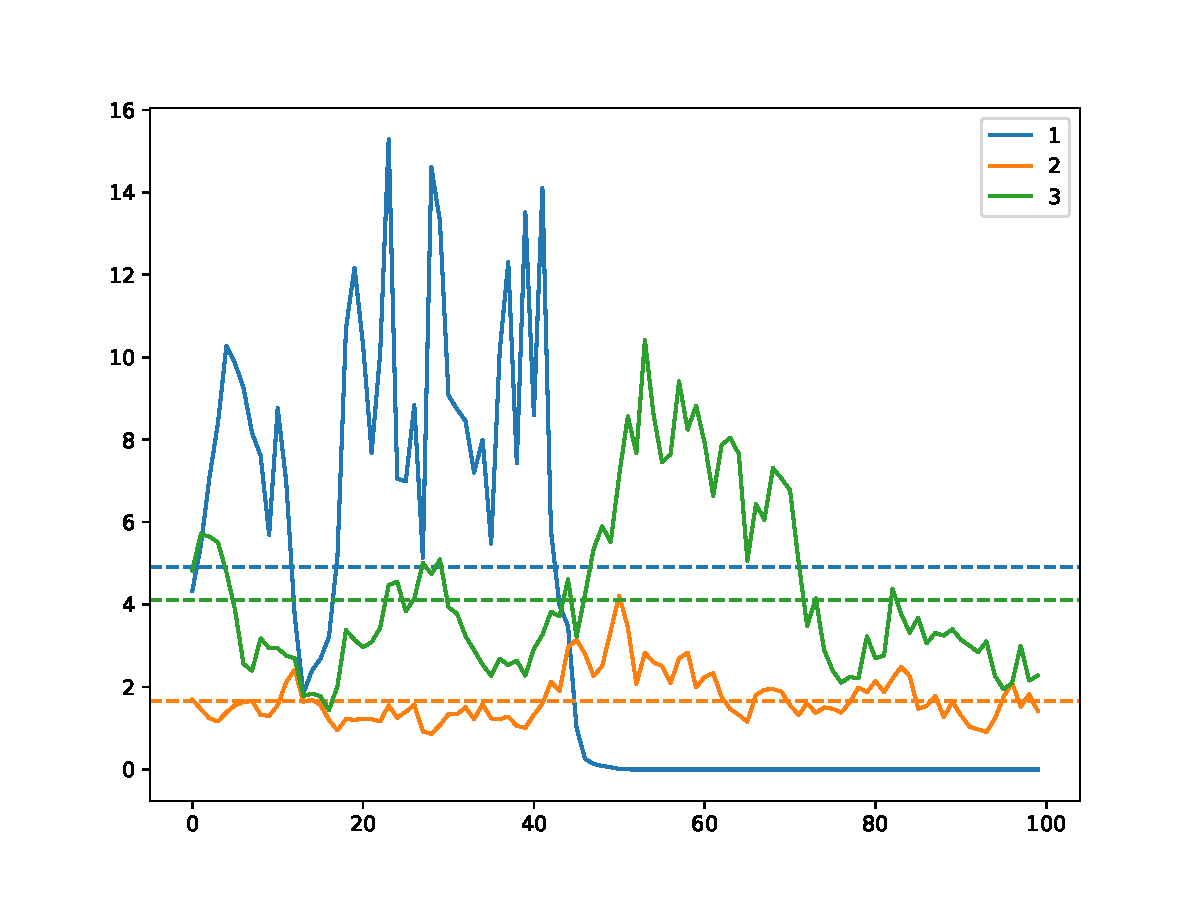
\includegraphics[width = 0.35\linewidth]{figures/chapter_3/discreteTS_species_3_noise_0.2_iter_1.pdf}}
\hfill
\subfigure[]{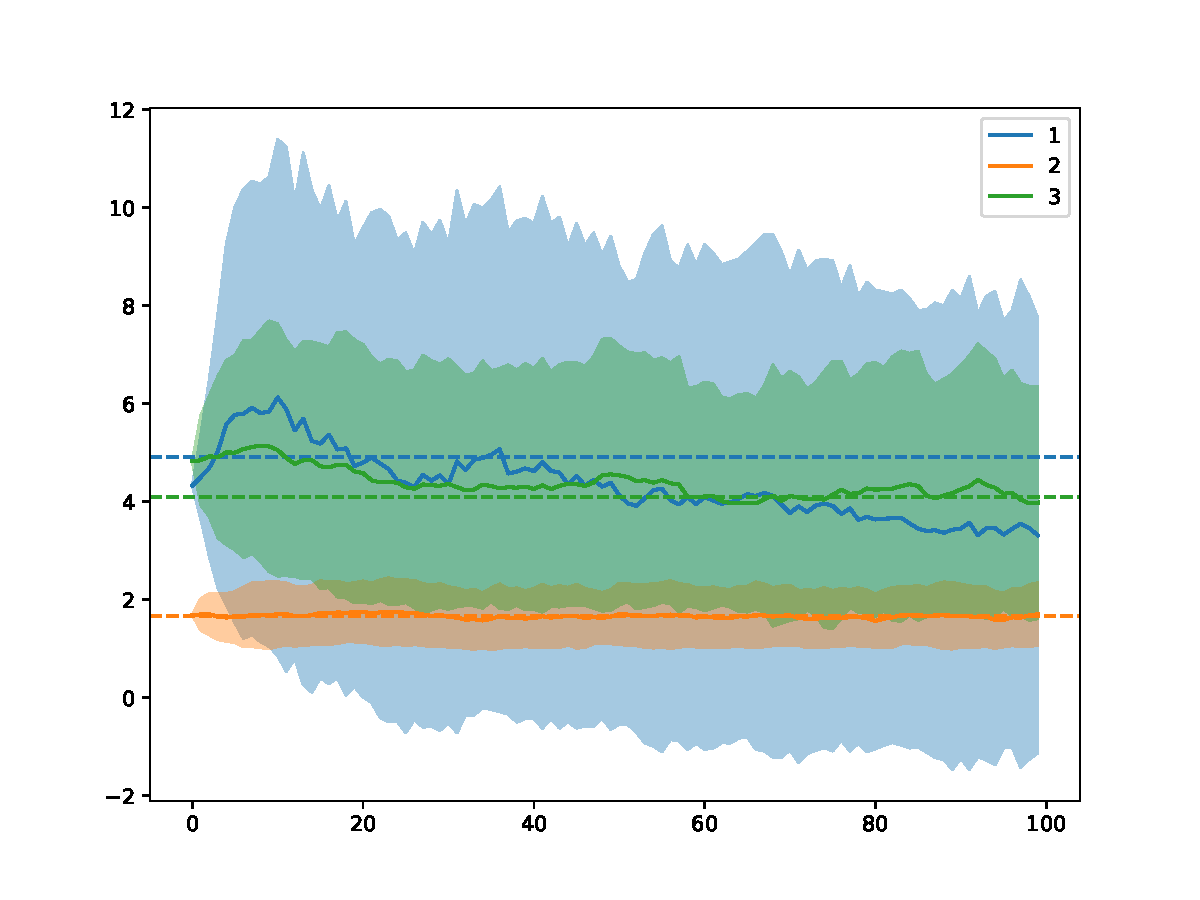
\includegraphics[width = 0.35\linewidth]{figures/chapter_3/discreteTS_species_3_noise_0.2_iter_200.pdf}}
\caption{Parameters are $\sigma = 0.2$. The figure (c) is the mean and std deviation of process repeated $200$ times with fixed initiali conditions. Figure (b) is a typical realization of the process. }
\end{figure}



\section{Results on mice data}